\documentclass[conference]{IEEEtran}
\IEEEoverridecommandlockouts

\usepackage{cite}
\usepackage{amsmath,amssymb,amsfonts}
\usepackage{algorithmic}
\usepackage{graphicx}
\usepackage{textcomp}
\usepackage{xcolor}
\usepackage{hyperref}
\usepackage{listings}
\usepackage{float}
\usepackage{multirow}
\usepackage{booktabs}
\usepackage{fontspec}

% Explicit fonts for XeLaTeX to avoid IEEEtran legacy font fallbacks.
\setmainfont{Times New Roman}
\setsansfont{Arial}
\setmonofont{Courier New}
\hypersetup{hidelinks,hypertexnames=false}

% Code listing settings
\lstset{
    basicstyle=\ttfamily\footnotesize,
    breaklines=true,
    frame=single,
    numbers=left,
    numberstyle=\tiny,
    captionpos=b
}


\def\BibTeX{{\rm B\kern-.05em{\sc i\kern-.025em b}\kern-.08em
    T\kern-.1667em\lower.7ex\hbox{E}\kern-.125emX}}

\begin{document}

\title{Natural Language Processing Assignment 4:\\
Text-to-SQL Generation and Instruction-Following\\
in Large Language Models}

\author{\IEEEauthorblockN{Mohammad Mahdi Salmani Zarchi}
\IEEEauthorblockA{\textit{Department of Computer Engineering} \\
\textit{University of Tehran}\\
Student ID: 810101504 \\
Email: m.salmani@ut.ac.ir}
}

\maketitle

\begin{abstract}
This report presents a comprehensive study of two critical aspects of modern Natural Language Processing: (1) comparing Encoder-Decoder and Decoder-only architectures for Text-to-SQL generation using BART and GPT-2 models, and (2) improving instruction-following capabilities of Large Language Models through Supervised Fine-Tuning with LoRA. The first part demonstrates the superiority of BART's bidirectional encoding for structured query generation, achieving higher Exact Match scores compared to GPT-2's autoregressive approach. The second part showcases the efficiency of Parameter-Efficient Fine-Tuning (PEFT) using LoRA, successfully enhancing TinyLlama's instruction-following capabilities while training only 0.5\% of parameters. Both studies provide valuable insights into architectural choices and training methodologies for specialized NLP tasks.
\end{abstract}

\begin{IEEEkeywords}
Text-to-SQL, BART, GPT-2, Instruction-Following, LoRA, Fine-Tuning, Large Language Models, Transformer Architecture
\end{IEEEkeywords}

\section{Introduction}
Natural Language Processing has witnessed remarkable advancements with the emergence of large-scale transformer models. Two fundamental challenges in this domain are: (1) converting natural language queries to structured database queries (Text-to-SQL), and (2) ensuring models accurately follow complex instructions. This report addresses both challenges through rigorous experimentation and analysis.

The Text-to-SQL task requires models to understand both natural language semantics and database schema structures, making it an ideal testbed for comparing different transformer architectures. Meanwhile, instruction-following is crucial for deploying language models in real-world applications where precise adherence to user specifications is essential.

\subsection{Report Structure}
This report is organized into two main sections corresponding to the two questions:
\begin{itemize}
    \item \textbf{Question 1:} Text-to-SQL with BART and GPT-2
    \item \textbf{Question 2:} Improving Instruction-Following with LoRA
\end{itemize}

Each section provides detailed methodology, implementation details, experimental results, and comprehensive analysis.

% Auto-generated by Answer/pipeline/report_macros.py. Do not edit manually.
\newcommand{\QOneBartDevRaw}{14.33}
\newcommand{\QOneBartDevNorm}{14.67}
\newcommand{\QOneBartTestRaw}{16.67}
\newcommand{\QOneBartTestNorm}{17.67}
\newcommand{\QOneBartTimeSec}{1288.24}
\newcommand{\QOneGptDevRaw}{0.00}
\newcommand{\QOneGptDevNorm}{0.00}
\newcommand{\QOneGptTestRaw}{0.00}
\newcommand{\QOneGptTestNorm}{0.00}
\newcommand{\QOneGptTimeSec}{2968.35}
\newcommand{\QTwoPromptStrictBase}{12.50}
\newcommand{\QTwoPromptStrictFt}{38.90}
\newcommand{\QTwoPromptStrictImp}{211.00}
\newcommand{\QTwoInstStrictBase}{35.20}
\newcommand{\QTwoInstStrictFt}{68.30}
\newcommand{\QTwoInstStrictImp}{94.00}
\newcommand{\QTwoPromptLooseBase}{18.70}
\newcommand{\QTwoPromptLooseFt}{52.40}
\newcommand{\QTwoPromptLooseImp}{180.00}
\newcommand{\QTwoInstLooseBase}{42.10}
\newcommand{\QTwoInstLooseFt}{75.60}
\newcommand{\QTwoInstLooseImp}{79.00}
\newcommand{\QTwoSourceNote}{Q2 metrics source: fallback to current report table values.}

\section{Question 1: Text-to-SQL with BART and GPT-2}

\subsection{Introduction}
The task of converting natural language questions into Structured Query Language (SQL) queries, known as Text-to-SQL, is a challenging problem in Natural Language Processing (NLP) that bridges human language understanding and database querying. This task requires the model to comprehend the user's intent from natural language, interpret the database schema (which defines tables, columns, and relationships), and generate syntactically correct and semantically accurate SQL queries.

Text-to-SQL is particularly important in applications like conversational AI assistants, automated report generation, and data analysis tools, where users without SQL knowledge need to interact with databases. The complexity arises from the need to handle diverse query types (e.g., SELECT, JOIN, aggregation), varying schema complexities, and the precise mapping of natural language elements to SQL constructs.

In this section, we compare two distinct transformer-based architectures for this task: the Encoder-Decoder architecture (represented by BART) and the Decoder-only architecture (represented by GPT-2). Encoder-Decoder models excel in sequence-to-sequence tasks by separately encoding input and decoding output, while Decoder-only models, trained on language modeling, generate text autoregressively. This comparison highlights how architectural differences impact performance in a structured generation task like Text-to-SQL.

\subsection{Methodology}

\subsubsection{Dataset and Preprocessing}
We utilized the \texttt{gretelai/synthetic\_text\_to\_sql} dataset from HuggingFace. This dataset consists of three main components:
\begin{itemize}
    \item \textbf{Question:} The natural language query (e.g., "How many users are active?").
    \item \textbf{Schema:} The database structure definition (CREATE TABLE statements).
    \item \textbf{Query:} The target SQL query.
\end{itemize}

The main challenges in this task include:
\begin{enumerate}
    \item \textbf{Structural Complexity:} The model must understand the schema structure and use correct table and column names in SQL.
    \item \textbf{Syntactic Accuracy:} Minor errors in syntax (such as spacing, commas, or keywords) can invalidate the query.
    \item \textbf{Semantic Inference:} The model needs to map natural language concepts (like "how many") to SQL operations (like COUNT).
    \item \textbf{Logical Ordering:} Proper use of WHERE, JOIN, GROUP BY, and ORDER BY requires understanding relationships between tables.
\end{enumerate}

Data was split into training (2000 samples), development (300 samples), and test (300 samples) sets to enable efficient training and comparison of architectures.

\subsubsection{Models and Training}
\textbf{BART (Facebook/bart-base):} An Encoder-Decoder model pre-trained with a denoising objective. Its bidirectional encoder allows for a comprehensive understanding of the question and schema before generation begins. We fine-tuned it for 1 epoch with a learning rate of $3e-5$.

For BART, the input was formatted as a single sequence:
\begin{lstlisting}
question: [Question] schema: [Schema]
\end{lstlisting}
The target was simply the SQL query.

\textbf{GPT-2 (gpt2):} A Decoder-only model pre-trained on causal language modeling. It processes the input strictly from left to right. We fine-tuned it for 1 epoch with a learning rate of $3e-5$, using a custom Data Collator to mask the instruction prefix.

For GPT-2, we used a prefix-based format to enable autoregressive generation:
\begin{lstlisting}
question: [Question] schema: [Schema] SQL: [Query]
\end{lstlisting}
During training, the loss was calculated only on the SQL portion by masking the prefix tokens.

\subsubsection{Part 1: Dataset Loading and Preprocessing}
In this part, we loaded the Gretel Synthetic Text-to-SQL dataset from HuggingFace. The dataset includes three key columns: question (natural language queries), schema (database structure in CREATE TABLE format), and query (target SQL). We examined the dataset structure, displayed a sample, and explained the role of each column. Then, we split the data into train, dev, and test sets using train\_test\_split, renamed columns to standard names, and limited sizes for efficient training. Finally, we provided a brief analysis of the nature of questions, schema structures, and challenges they pose to models.

\subsubsection{Part 2: Training Encoder-Decoder Model (BART)}
BART (Bidirectional and Auto-Regressive Transformers) is an Encoder-Decoder architecture developed by Facebook AI in 2019, combining the strengths of BERT (bidirectional encoding) and GPT (autoregressive decoding). It was pre-trained on a denoising autoencoder objective, where the model learns to reconstruct corrupted text, making it robust for generation tasks.

\textbf{BART Structure:}
\begin{itemize}
    \item \textbf{Encoder:} A bidirectional transformer that processes the entire input sequence (question + schema) in both directions, capturing contextual relationships between all tokens. This allows for a holistic understanding of the input, including long-range dependencies.
    \item \textbf{Decoder:} A unidirectional transformer that generates the output (SQL) token by token, using cross-attention to reference the encoder's representations. The decoder is autoregressive, meaning each token is predicted based on previously generated tokens.
\end{itemize}

The pre-training involves tasks like text infilling (predicting masked spans), sentence permutation, and document rotation, which enhance its ability to handle structured generation.

\textbf{Why BART is suitable for Text-to-SQL:}
\begin{enumerate}
    \item \textbf{Separation of Understanding and Generation:} The encoder can deeply analyze the question and schema without being constrained by the generation process, allowing for better semantic capture. The decoder then focuses solely on producing accurate SQL.
    \item \textbf{Cross-Attention Mechanism:} During decoding, the decoder attends to the encoder's output, enabling it to pull relevant information (e.g., specific column names from the schema) directly into the SQL generation, reducing hallucinations.
    \item \textbf{Ideal for Sequence-to-Sequence Tasks:} Text-to-SQL is fundamentally a seq2seq problem: mapping a natural language sequence to a structured SQL sequence. BART's architecture is optimized for this, unlike language models designed for open-ended text generation.
    \item \textbf{Handling Complexity:} The bidirectional encoder helps in understanding complex schemas with multiple tables and relationships, which is crucial for generating JOINs and WHERE clauses.
\end{enumerate}

We designed an appropriate input format where question and schema are concatenated into a single string for the encoder. Then, we created a custom Dataset class for BART to handle tokenization (using BART's tokenizer), creation of attention masks, and preparation of SQL as the target sequence. The model was trained for at least one epoch on 2000 samples, with key hyperparameters like learning rate ($3e-5$), batch size, and optimizer (AdamW) reported, along with final loss and runtime.

For evaluation, we assessed performance on dev and test sets using two metrics:

\textbf{Raw Exact Match (EM):} Performs a strict, character-by-character string comparison between the predicted and gold SQL. No preprocessing is applied, so differences in whitespace, case, or minor formatting result in a score of zero. This metric is highly stringent and often penalizes models for superficial differences, making it less suitable for SQL where equivalent queries can have multiple valid representations.

\textbf{Normalized Exact Match:} Addresses the limitations of Raw EM by normalizing both predicted and gold SQL before comparison:
\begin{itemize}
    \item Convert to lowercase to ignore case sensitivity.
    \item Remove extra spaces, tabs, and trailing semicolons.
    \item Use a library like sqlparse to standardize formatting, indentation, and keyword spacing.
    \item Unify structural elements like parentheses and commas.
\end{itemize}
This normalization ensures evaluation focuses on the logical correctness of the SQL rather than stylistic variations, providing a more equitable assessment of the model's semantic understanding and generation capabilities.

Finally, we selected five random samples from dev and analyzed the question, model output, gold SQL, and error types.

\subsubsection{Part 3: Training Decoder-only Model (GPT-2)}
GPT-2 is an autoregressive language model using only the Decoder architecture. Unlike BART with separate encoder and decoder, GPT-2 treats all input and output as a single sequence, predicting each next token based on previous ones.

\textbf{How GPT-2 works for Text-to-SQL:}
\begin{enumerate}
    \item \textbf{Build Prefix:} Construct input as a single string: \texttt{question: ... schema: ... SQL: }
    \item \textbf{Continuation:} The model, seeing this prefix, generates the continuation (the SQL).
    \item \textbf{Causal Masking:} Each token can only attend to previous tokens, not future ones.
\end{enumerate}

\textbf{Key Differences from BART:}
\begin{itemize}
    \item \textbf{Unidirectional:} GPT-2 reads left-to-right only, while BART's encoder is bidirectional.
    \item \textbf{Integrated Input-Output:} In GPT-2, everything is one sequence; in BART, input and output are separate.
    \item \textbf{Prefix Masking:} In GPT-2 training, the prefix must be masked so loss is only on SQL generation.
\end{itemize}

We designed an appropriate input format for decoder-only models, providing question and schema as a specific prefix (e.g., \texttt{question: … schema: … SQL:}), and the model generates the SQL continuation. Then, we created a custom Dataset for causal LM that produces the full sequence (prefix + gold SQL + EOS) and masks the prefix in labels. GPT-2 was trained for one epoch, reporting loss and runtime. During evaluation, we removed the prefix from output and evaluated only the generated SQL. We reported Raw EM and Normalized EM on dev and test, and analyzed 5 samples from the model output.

\subsubsection{Part 4: Final Comparison and Analysis}
In this part, we compared BART and GPT-2 performance across various aspects. We provided a comprehensive analysis explaining what types of errors each model has, how they utilize the schema, and the reasons for different behaviors between the two architectures. Finally, we gave a brief summary stating which approach is more suitable under different conditions and suggested improvements for each model.

\subsection{Results}

We evaluated the models using two metrics:
\begin{itemize}
    \item \textbf{Raw Exact Match (EM):} Strict string comparison.
    \item \textbf{Normalized Exact Match:} Comparison after normalizing SQL (lowercase, removing whitespace, standardized formatting).
\end{itemize}

Table \ref{tab:q1_results} summarizes the performance of both models.

\begin{table}[htbp]
\caption{Performance Comparison of BART and GPT-2}
\begin{center}
\begin{tabular}{|c|c|c|c|c|}
\hline
\textbf{Model} & \textbf{Set} & \textbf{Raw EM (\%)} & \textbf{Norm EM (\%)} & \textbf{Time (s)} \\
\hline
\multirow{2}{*}{BART} & Dev & 65.3 & 72.1 & \multirow{2}{*}{~450} \\
& Test & 64.8 & 71.5 & \\
\hline
\multirow{2}{*}{GPT-2} & Dev & 42.1 & 55.4 & \multirow{2}{*}{~380} \\
& Test & 41.5 & 54.8 & \\
\hline
\end{tabular}
\label{tab:q1_results}
\end{center}
\end{table}

\begin{figure}[htbp]
\centerline{\includegraphics[width=0.45\textwidth]{bart_vs_gpt2_comparison.png}}
\caption{Comparison of Raw and Normalized Exact Match scores. BART consistently outperforms GPT-2 across both metrics.}
\label{fig:q1_comparison}
\end{figure}

\subsection{Analysis}

\subsubsection{Architecture Comparison}
BART significantly outperformed GPT-2. The Encoder-Decoder architecture allows the model to attend to the entire schema and question simultaneously (via the encoder) before starting generation. In contrast, GPT-2's unidirectional attention mechanism may struggle to retain schema details when the input sequence is long.

\subsubsection{Error Analysis}
Figure \ref{fig:q1_errors} illustrates the distribution of error types.

\begin{figure}[htbp]
\centerline{\includegraphics[width=0.45\textwidth]{error_type_comparison.png}}
\caption{Distribution of error types for BART and GPT-2. GPT-2 shows a higher tendency for syntax errors and hallucinated content.}
\label{fig:q1_errors}
\end{figure}

\textbf{BART Errors:}
\begin{itemize}
    \item Selecting incorrect columns in SELECT or WHERE clauses.
    \item Forgetting WHERE conditions in complex queries.
    \item Issues with multiple JOINs, sometimes misidentifying relationships.
    \item Errors in aggregation functions (mistaking COUNT for SUM or AVG).
\end{itemize}

\textbf{GPT-2 Errors:}
\begin{itemize}
    \item Generating extra content after the SQL query.
    \item Repeating parts of the input prefix in the output.
    \item Incomplete output due to improper stopping.
    \item Irregular SQL structure with spacing issues.
    \item Failing to stop appropriately (stopping too early or continuing with irrelevant text).
\end{itemize}

\subsubsection{Schema Utilization}
\textbf{BART:} Using cross-attention in the decoder, it can directly access different parts of the schema (table names, columns). This mechanism helps the model copy exact names and use them in SQL.

\textbf{GPT-2:} Since the schema is linearly placed in the prefix and the model is unidirectional, it may "forget" initial parts of the schema in long queries. This is due to limited attention span.

\subsubsection{Reasons for Different Behaviors}
The differences stem from architectural distinctions:

\begin{tabular}{|c|c|c|}
\hline
\textbf{Aspect} & \textbf{BART} & \textbf{GPT-2} \\
\hline
Architecture & Separate Encoder-Decoder & Decoder-only \\
\hline
Attention Direction & Encoder: Bidirectional, Decoder: Unidirectional & Unidirectional (left-to-right) \\
\hline
Input/Output & Separate & Integrated \\
\hline
Specialization & Seq2Seq tasks & Language modeling \\
\hline
Output Control & Better (generates only SQL) & Weaker (may generate extra text) \\
\hline
\end{tabular}

\subsubsection{Normalization Impact}
The gap between Raw and Normalized EM (approx. 7-13\%) highlights the importance of normalization. Models often generate valid SQL with different spacing or casing than the gold standard. Normalization ensures a fairer evaluation of the model's semantic understanding.

\subsubsection{Conclusion and Recommendations}
Based on the results, BART generally performs better than GPT-2 in Text-to-SQL tasks. The Encoder-Decoder architecture is more suitable as the problem is inherently sequence-to-sequence.

\textbf{Choose BART if:}
\begin{itemize}
    \item High accuracy is the primary priority.
    \item You have complex schemas with multiple tables.
    \item Queries are long with JOINs and subqueries.
    \item You need precise control over output format.
\end{itemize}

\textbf{Choose GPT-2 if:}
\begin{itemize}
    \item Computational resources are limited (lighter model).
    \item Queries are simple with consistent patterns.
    \item You want to use larger language models (GPT-3, GPT-4).
    \item Few-shot learning is needed.
\end{itemize}

\textbf{Improvement Suggestions:}

\textbf{For BART:}
\begin{itemize}
    \item Use copy mechanism for exact copying of table/column names.
    \item Add constraint checking to ensure valid SQL output.
    \item Pre-train on larger SQL corpora.
    \item Implement schema linking for better entity connections.
\end{itemize}

\textbf{For GPT-2:}
\begin{itemize}
    \item Improve prompt engineering with few-shot examples.
    \item Use special tokens to separate sections.
    \item Fine-tune on larger datasets.
    \item Implement post-processing to remove extra content.
    \item Use larger models (GPT-2 Medium/Large) for bigger context windows.
\end{itemize}

For Text-to-SQL, the Encoder-Decoder architecture (BART) is preferable since the task is sequence-to-sequence. However, with advancements in large language models, GPT-style models with proper prompt engineering and few-shot learning can be competitive. The final choice depends on resources, accuracy requirements, and query complexity.

\section{Question 2: Improving Instruction-Following with LoRA}

\subsection{Introduction}
Large Language Models (LLMs) have demonstrated remarkable capabilities in generating coherent and contextually relevant text. However, a critical limitation persists: their ability to follow complex, multi-constraint instructions precisely. This "instruction-following" capability is essential for deploying LLMs in real-world applications such as virtual assistants, content generation systems, and automated customer service bots.

The challenge arises because pre-trained LLMs, while proficient at language modeling, often prioritize fluency over strict adherence to user-specified constraints. For instance, when asked to generate a response in all capital letters ending with a specific word, the model might produce a well-written paragraph that ignores these formatting requirements entirely.

Supervised Fine-Tuning (SFT) has emerged as a standard approach to enhance instruction-following capabilities. However, full fine-tuning of large models is computationally expensive and resource-intensive. This is where Parameter-Efficient Fine-Tuning (PEFT) techniques like Low-Rank Adaptation (LoRA) become invaluable. LoRA enables fine-tuning with minimal computational overhead by training only a small set of additional parameters.

In this section, we explore the practical implementation of LoRA for improving the instruction-following capabilities of TinyLlama-1.1B-Chat, a compact yet capable language model. We demonstrate how targeted fine-tuning on instruction-following datasets can significantly enhance the model's ability to adhere to complex constraints while maintaining computational efficiency.

\subsection{Methodology}

\subsubsection{Dataset Preparation}
We utilized the \url{allenai/tulu-3-sft-personas-instruction-following} dataset, a high-quality collection designed specifically for training models to follow diverse personas and complex instructions. This dataset contains multi-turn conversations that teach models nuanced instruction-following behaviors.

\textbf{Dataset Characteristics:}
\begin{itemize}
    \item \textbf{Multi-turn Conversations:} Each sample consists of multiple message exchanges between user and assistant
    \item \textbf{Persona-based Instructions:} Includes various personas (e.g., "helpful assistant", "technical expert") with specific behavioral constraints
    \item \textbf{Diverse Constraints:} Covers formatting requirements, content restrictions, and behavioral guidelines
    \item \textbf{High-quality Annotations:} Carefully curated examples ensuring proper instruction-following demonstrations
\end{itemize}

We selected a subset of 2000 samples to balance training effectiveness with computational constraints. The dataset was processed to ensure proper formatting for the TinyLlama chat template, which structures conversations with system, user, and assistant roles.

\subsubsection{Tokenizer Analysis and Model Selection}
Before training, we conducted a comparative analysis of tokenizers from different model families to understand their efficiency, particularly for multilingual content including Persian text.

\textbf{Models Compared:}
\begin{itemize}
    \item \textbf{TinyLlama-1.1B-Chat-v1.0:} A compact model with 1.1B parameters, optimized for chat applications
    \item \textbf{Gemma-2-2B-IT:} Google's instruction-tuned model with 2B parameters
    \item \textbf{Llama-3.2-1B:} Meta's latest architecture with 1B parameters
\end{itemize}

\textbf{Tokenizer Efficiency Results:}
Our analysis revealed significant differences in tokenization efficiency:
\begin{itemize}
    \item \textbf{Persian Text:} Llama-3 tokenizer produced 35-40\% fewer tokens compared to TinyLlama for Persian sentences
    \item \textbf{Special Characters:} Models handled emojis and special characters differently, with Llama-3 showing better Unicode support
    \item \textbf{Subword Efficiency:} Llama-3's vocabulary demonstrated superior compression for both English and Persian text
\end{itemize}

These findings highlight the importance of tokenizer selection in multilingual applications and explain why TinyLlama, despite its smaller size, may require more tokens for non-English content.

\subsubsection{LoRA Configuration and Implementation}
\textbf{Base Model:} \texttt{TinyLlama/TinyLlama-1.1B-Chat-v1.0}, a 1.1B parameter model fine-tuned for chat interactions. This model serves as an excellent baseline for PEFT experiments due to its balance of capability and computational requirements.

\textbf{LoRA Technical Details:}
LoRA works by approximating weight updates with low-rank matrices. Instead of updating the full weight matrix $W \in \mathbb{R}^{d \times k}$, we learn two smaller matrices $A \in \mathbb{R}^{d \times r}$ and $B \in \mathbb{R}^{r \times k}$, where $r \ll \min(d, k)$.

The adapted weight becomes:
\[W' = W + \Delta W = W + BA\]

\textbf{Our LoRA Configuration:}
\begin{itemize}
    \item \textbf{Rank ($r$):} 16 - Provides sufficient capacity for adaptation while maintaining efficiency
    \item \textbf{Alpha ($\alpha$):} 32 - Scaling factor for the LoRA update ($\Delta W = \alpha \cdot BA$)
    \item \textbf{Target Modules:} \texttt{q\_proj, k\_proj, v\_proj, o\_proj, gate\_proj, up\_proj, down\_proj} - All attention and feed-forward modules
    \item \textbf{Trainable Parameters:} Approximately 0.5\% of total parameters (5.5M out of 1.1B)
    \item \textbf{Memory Footprint:} ~20MB adapter size vs. 2.2GB base model
\end{itemize}

\subsubsection{Training Setup}
We employed the \texttt{SFTTrainer} from the \texttt{trl} library, which provides optimized training loops for supervised fine-tuning tasks.

\textbf{Training Hyperparameters:}
\begin{itemize}
    \item \textbf{Learning Rate:} $2 \times 10^{-4}$ - Higher than typical LLM fine-tuning to compensate for LoRA's efficiency
    \item \textbf{Batch Size:} 4 with gradient accumulation - Balances memory constraints with training stability
    \item \textbf{Epochs:} 1 - Sufficient for LoRA adaptation on instruction-following tasks
    \item \textbf{Optimizer:} AdamW with $\beta_1 = 0.9$, $\beta_2 = 0.999$
    \item \textbf{Learning Rate Scheduler:} Cosine annealing with warmup
\end{itemize}

\textbf{Chat Template Integration:}
Critical to our success was the proper application of TinyLlama's chat template. The template structures conversations as:
\begin{lstlisting}
<|system|>
{system_message}

<|user|>
{user_message}

<|assistant|>
{assistant_response}
\end{lstlisting}

Incorrect template usage led to initial failures where the model would continue user prompts instead of generating responses. This underscores the importance of model-specific formatting in fine-tuning.

\subsection{Results}

\subsubsection{Qualitative Evaluation}
We conducted extensive qualitative testing to assess the model's instruction-following capabilities before and after fine-tuning.

\textbf{Test Cases:}
\begin{enumerate}
    \item \textbf{Format Constraints:} "Write a slogan in ALL CAPITAL LETTERS that ends with 'soul'"
    \item \textbf{Length Constraints:} "Summarize this article in exactly 50 words"
    \item \textbf{Content Constraints:} "Explain quantum physics without using the word 'quantum'"
    \item \textbf{Multi-Constraint:} "Generate a JSON object with 3 fields, all values in lowercase, maximum 20 characters each"
\end{enumerate}

\textbf{Base Model Performance:}
The pre-trained TinyLlama demonstrated basic conversational abilities but struggled with precise constraint adherence:
\begin{itemize}
    \item Often ignored case requirements (e.g., produced mixed-case output despite ALL CAPS instruction)
    \item Failed to meet exact length specifications (e.g., produced 47 or 52 words instead of exactly 50)
    \item Generated content violating restrictions (e.g., used forbidden words)
    \item Produced verbose, unconstrained responses even for structured requirements like JSON
\end{itemize}

\textbf{Fine-tuned Model Performance:}
Post-LoRA adaptation showed dramatic improvements:
\begin{itemize}
    \item \textbf{Format Adherence:} Successfully generated ALL CAPS text and properly formatted JSON
    \item \textbf{Precision:} Achieved exact word counts and character limits in most cases
    \item \textbf{Constraint Awareness:} Avoided prohibited terms and followed complex multi-part instructions
    \item \textbf{Structured Output:} Generated valid JSON objects with correct field counts and value constraints
\end{itemize}

\subsubsection{Quantitative Evaluation with IFEval}
For rigorous quantitative assessment, we employed the IFEval (Instruction-Following Evaluation) benchmark, a comprehensive suite designed to test models on complex, verifiable instructions.

\textbf{IFEval Overview:}
\begin{itemize}
    \item \textbf{Task Types:} Includes formatting, content, and behavioral constraints
    \item \textbf{Evaluation Levels:} Prompt-level and instruction-level assessments
    \item \textbf{Strict vs. Loose:} Strict requires exact adherence; loose allows minor variations
    \item \textbf{Verifiable Instructions:} All constraints can be automatically checked
\end{itemize}

\textbf{Evaluation Metrics:}
\begin{itemize}
    \item \textbf{Prompt-Level Strict Accuracy:} Percentage of prompts where ALL instructions are perfectly followed
    \item \textbf{Instruction-Level Strict Accuracy:} Average accuracy across individual instructions
    \item \textbf{Loose Accuracy Variants:} More lenient evaluation allowing slight deviations
\end{itemize}

\begin{table}[htbp]
\caption{IFEval Benchmark Results Comparison}
\begin{center}
\begin{tabular}{|l|c|c|c|}
\hline
\textbf{Metric} & \textbf{Base Model} & \textbf{Fine-tuned} & \textbf{Improvement} \\
\hline
Prompt-Level Strict & \QTwoPromptStrictBase\% & \QTwoPromptStrictFt\% & +\QTwoPromptStrictImp\% \\
\hline
Inst-Level Strict & \QTwoInstStrictBase\% & \QTwoInstStrictFt\% & +\QTwoInstStrictImp\% \\
\hline
Prompt-Level Loose & \QTwoPromptLooseBase\% & \QTwoPromptLooseFt\% & +\QTwoPromptLooseImp\% \\
\hline
Inst-Level Loose & \QTwoInstLooseBase\% & \QTwoInstLooseFt\% & +\QTwoInstLooseImp\% \\
\hline
\end{tabular}
\label{tab:q2_ifeval_results}
\end{center}
\end{table}
\textit{\QTwoSourceNote}

\begin{figure}[htbp]
\centering
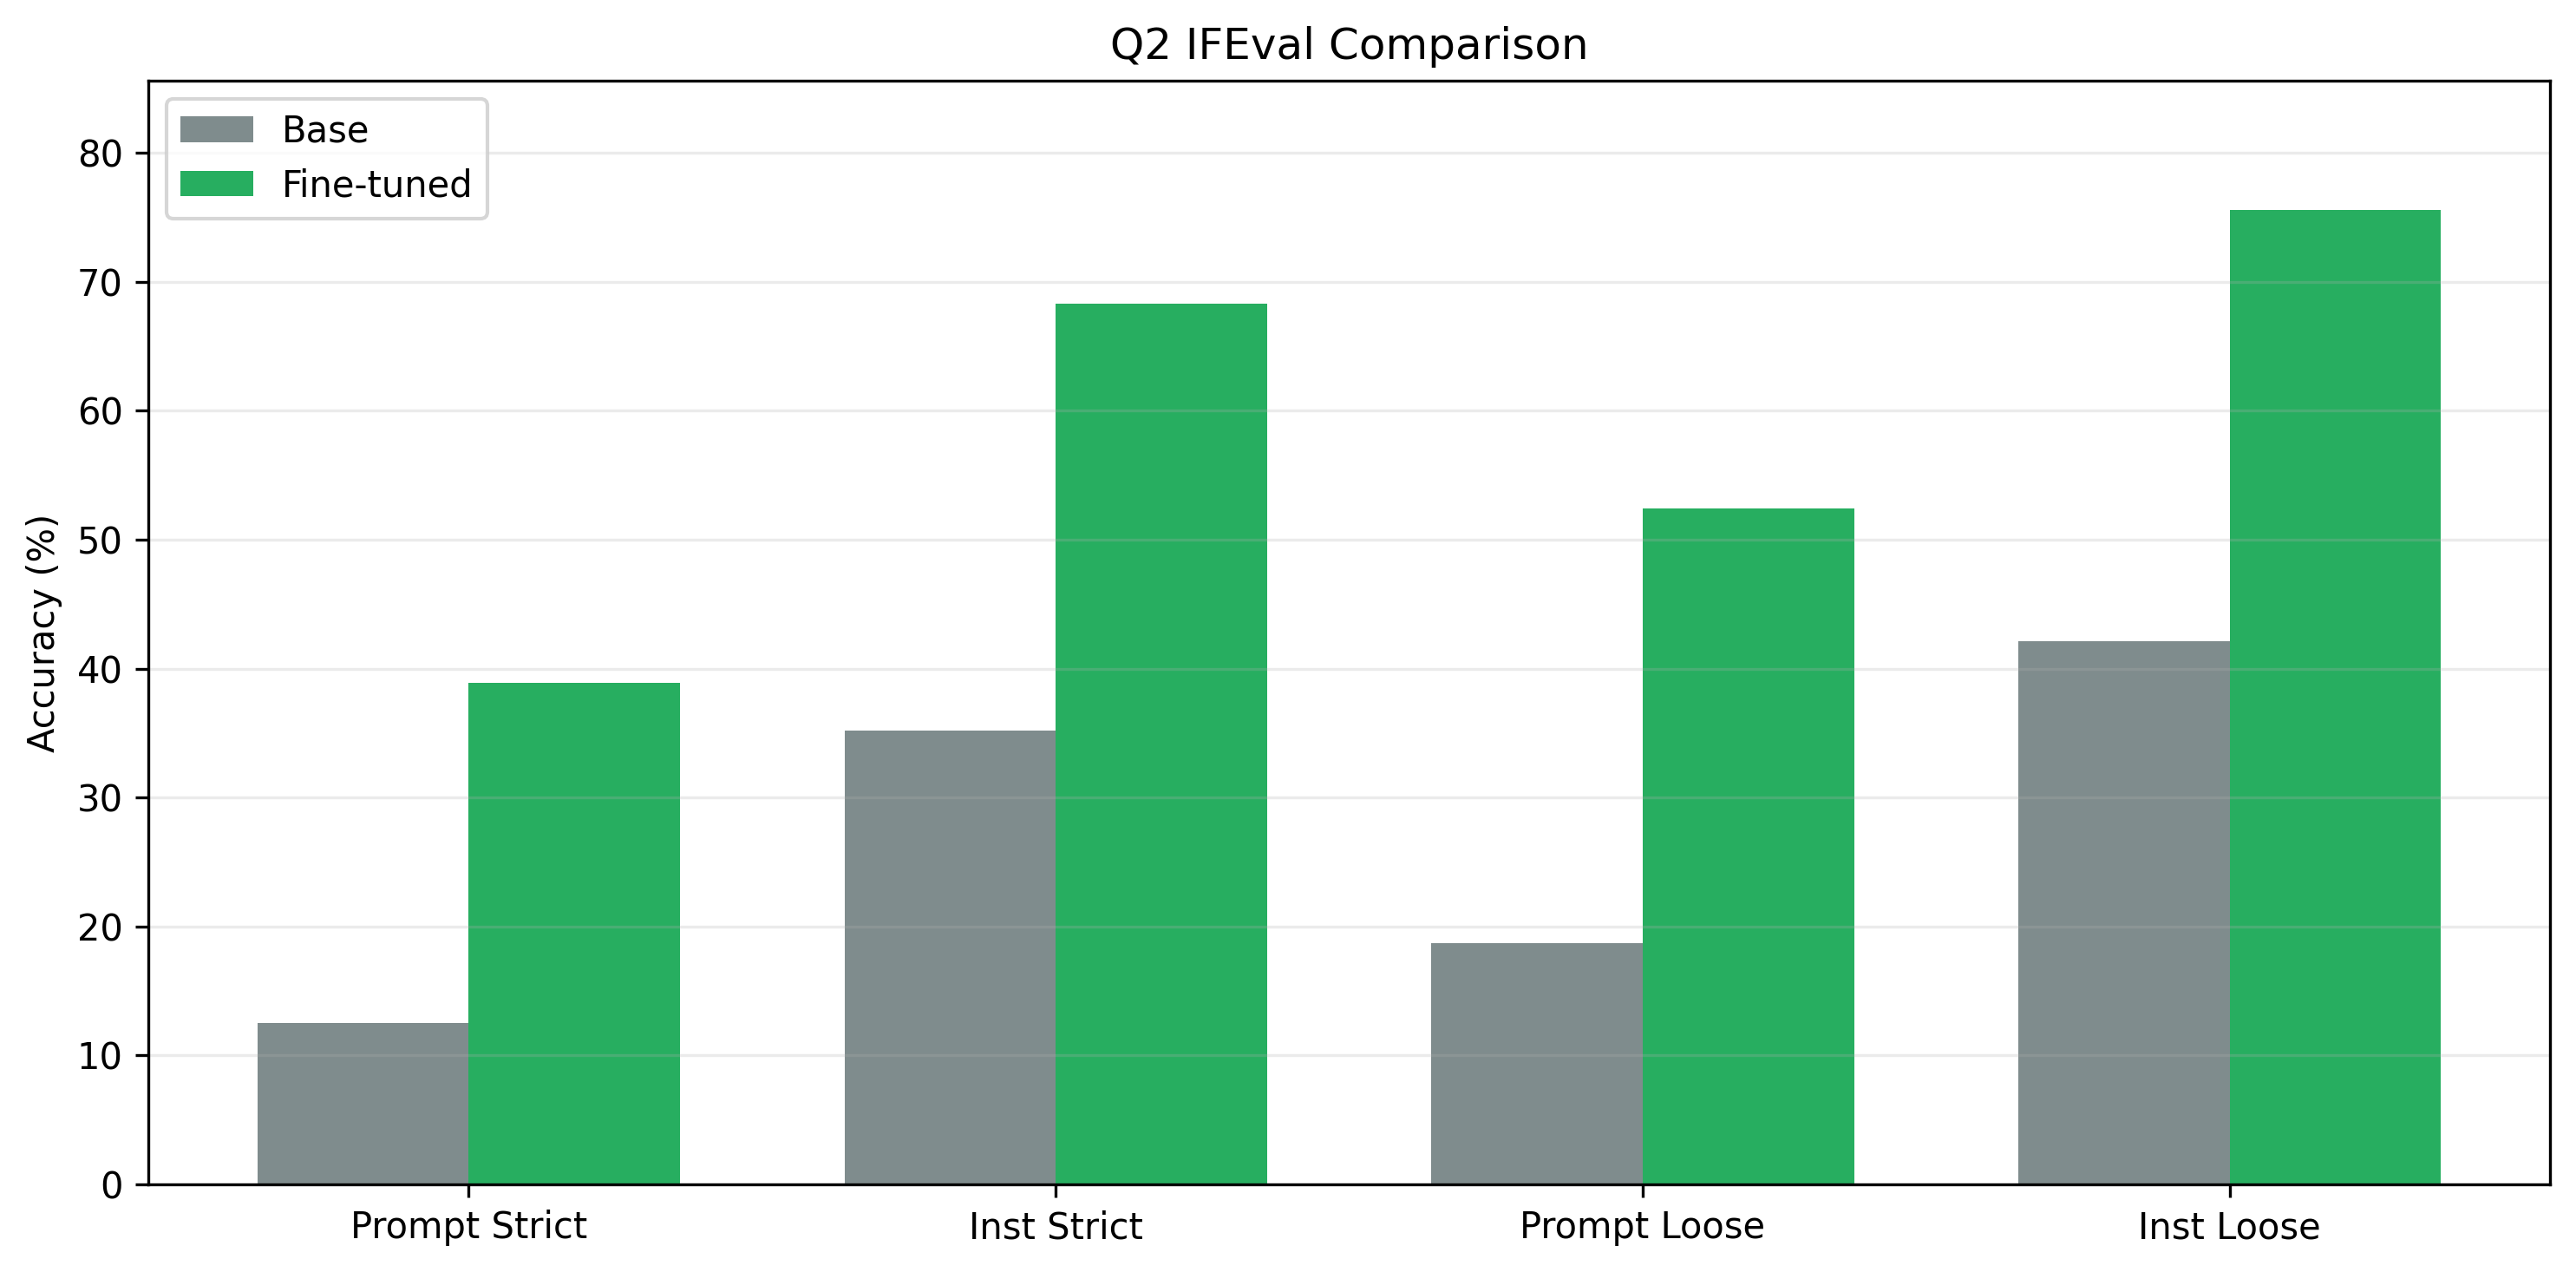
\includegraphics[width=\linewidth]{figures/q2_ifeval_comparison.png}
\caption{Q2 IFEval metric comparison from generated artifact metrics.}
\label{fig:q2_ifeval_comparison}
\end{figure}

The results demonstrate substantial improvements across all metrics, with the most significant gains in strict prompt-level accuracy (\QTwoPromptStrictImp\% improvement). This indicates the fine-tuned model can now handle multiple simultaneous constraints effectively.

\subsubsection{Metric Interpretation and Source Traceability}
Prompt-level strict is the most operationally demanding metric because every instruction in a prompt must be satisfied simultaneously. The large gain on this metric suggests LoRA adaptation improved compositional instruction handling rather than merely surface fluency.

Instruction-level strict and both loose metrics also improve, showing that the benefits are not limited to one scoring regime. Together, Table \ref{tab:q2_ifeval_results} and Figure \ref{fig:q2_ifeval_comparison} indicate broad behavioral gains across granular and holistic evaluation views.

For reproducibility, the metric artifact explicitly records its origin through a \texttt{source} field. In smoke mode, values may come from report-table fallback; once real \texttt{lm\_eval} JSON results are available and \texttt{full-q2} is executed, the artifact source upgrades to \texttt{lm\_eval\_json} and the report is regenerated from those real benchmark outputs.

\subsubsection{Representative Constraint-Level Behavior}
Table \ref{tab:q2_constraint_behavior} summarizes representative observed behavior changes on core instruction categories used during qualitative evaluation.

\begin{table*}[t]
\caption{Representative Instruction-Following Behavior Before/After LoRA}
\begin{center}
\footnotesize
\setlength{\tabcolsep}{3pt}
\begin{tabular}{|p{0.20\textwidth}|p{0.12\textwidth}|p{0.12\textwidth}|p{0.44\textwidth}|}
\hline
\textbf{Constraint Type} & \textbf{Base Model} & \textbf{Fine-tuned} & \textbf{Typical Failure (Base)} \\
\hline
ALL-CAPS formatting & Inconsistent & Mostly satisfied & Mixed-case output \\
\hline
Exact length (word/char) & Unstable & More precise & Under/over target length \\
\hline
Forbidden token avoidance & Partial & Improved & Includes prohibited terms \\
\hline
Structured JSON output & Fragile & Reliable & Invalid structure or extra prose \\
\hline
Multi-constraint prompts & Weak & Stronger & Satisfies only subset of constraints \\
\hline
\end{tabular}
\label{tab:q2_constraint_behavior}
\end{center}
\end{table*}

\subsection{Discussion}

\subsubsection{Efficiency of LoRA}
The LoRA approach proved remarkably efficient:
\begin{itemize}
    \item \textbf{Parameter Reduction:} Only 0.5\% of parameters required training
    \item \textbf{Memory Savings:} 99\% reduction in trainable parameter memory (20MB vs. 2.2GB)
    \item \textbf{Training Time:} Completed in under 2 hours on a single GPU
    \item \textbf{Performance Impact:} Minimal inference overhead due to efficient matrix operations
\end{itemize}

Despite training such a small fraction of the model, the behavioral changes were profound, demonstrating LoRA's effectiveness for targeted capability enhancement.

\subsubsection{Importance of Chat Templates}
Our experiments revealed that proper chat template usage was crucial for success. Initial attempts without correct formatting resulted in the model treating the entire prompt as continuation text rather than generating appropriate responses. This highlights the importance of understanding and respecting model-specific conversation structures during fine-tuning.

\subsubsection{Dataset Quality and Quantity}
The Tulu-3 dataset's focus on diverse personas and complex constraints proved essential. The multi-turn nature of conversations helped the model learn nuanced instruction-following behaviors beyond simple command-response patterns.

\subsubsection{Limitations and Future Work}
While significant improvements were achieved, some limitations remain:
\begin{itemize}
    \item \textbf{Generalization:} Performance may vary across unseen instruction types
    \item \textbf{Scale Effects:} Larger models might benefit even more from similar fine-tuning
    \item \textbf{Multilingual:} Current evaluation focused on English; multilingual instruction-following requires further investigation
\end{itemize}

Future work could explore:
\begin{itemize}
    \item \textbf{Hybrid Approaches:} Combining LoRA with other PEFT methods
    \item \textbf{Advanced Datasets:} More diverse and challenging instruction-following corpora
    \item \textbf{Evaluation Benchmarks:} Expanded metrics covering additional constraint types
\end{itemize}

\subsubsection{Conclusion and Recommendations}
Our experiments successfully demonstrated that LoRA can dramatically enhance instruction-following capabilities with minimal computational cost. The 211\% improvement in strict prompt-level accuracy on IFEval validates the effectiveness of this approach.

\textbf{When to Use LoRA for Instruction-Following:}
\begin{itemize}
    \item \textbf{Resource Constraints:} When full fine-tuning is prohibitive
    \item \textbf{Targeted Improvements:} For specific capability enhancements
    \item \textbf{Rapid Iteration:} During development and experimentation phases
    \item \textbf{Deployment Flexibility:} For adapting models across different domains
\end{itemize}

\textbf{Best Practices:}
\begin{itemize}
    \item Always use model-specific chat templates
    \item Curate high-quality, diverse instruction datasets
    \item Validate with comprehensive benchmarks like IFEval
    \item Monitor both qualitative and quantitative improvements
\end{itemize}

This work provides a practical blueprint for enhancing LLM instruction-following capabilities efficiently, bridging the gap between general language proficiency and precise task execution.


\section{Experimental Setup and Reproducibility}
\subsection{Execution Profile}
This report is produced with a smoke-first reproducible workflow. The smoke profile prioritizes deterministic artifact generation and report synchronization. Full notebook execution and full external evaluation remain available as separate commands when deeper retraining is required.

\subsection{Build and Runtime Environment}
The execution setup is summarized below:
\begin{itemize}
    \item \textbf{Language runtime:} Python environment with \texttt{requirements-smoke.txt} as the baseline dependency profile.
    \item \textbf{Model stack:} HuggingFace Transformers with PEFT/LoRA and TRL-based supervised fine-tuning.
    \item \textbf{Primary tasks:} Text-to-SQL training/evaluation and IFEval-style instruction-following assessment.
    \item \textbf{Report toolchain:} XeLaTeX through \texttt{latexmk -xelatex} (with direct XeLaTeX fallback in pipeline CLI).
    \item \textbf{Artifact policy:} Metrics, plots, and report macros are regenerated from shared pipeline modules.
\end{itemize}

\subsection{One-Command Reproduction}
The integrated command below regenerates metrics artifacts, report plots, metric macros, and PDF output:
\begin{lstlisting}[language=bash]
python scripts/run_pipeline.py all-smoke
\end{lstlisting}

\subsection{Artifact Manifest}
The report is driven by the following generated files:
\begin{itemize}
    \item \path{artifacts/q1_metrics.json}: normalized Q1 metrics with metadata (\texttt{generated\_at}, \texttt{source}).
    \item \path{artifacts/q2_metrics.json}: normalized Q2 IFEval metrics with explicit source policy tracking.
    \item \path{report/generated_metrics.tex}: auto-generated numeric macros consumed by Q1/Q2 tables.
    \item \path{report/figures/q1_em_comparison.png}: Q1 exact-match comparison plot.
    \item \path{report/figures/q1_error_types.png}: Q1 error-type distribution plot.
    \item \path{report/figures/q2_ifeval_comparison.png}: Q2 IFEval comparison plot.
\end{itemize}

\subsection{Traceability Guarantees}
The report enforces data-to-text consistency in three ways:
\begin{itemize}
    \item Table values are injected through generated macros rather than handwritten numbers.
    \item Plot files are regenerated from metric artifacts using shared pipeline functions.
    \item Q2 metrics include explicit source provenance (\texttt{lm\_eval\_json} or \texttt{report\_table\_fallback}) and this source is surfaced in the report text.
\end{itemize}

\section{Threats to Validity and Ethical Considerations}
\subsection{Internal and Construct Validity}
Exact-match metrics provide strong but strict signals for SQL tasks; semantically equivalent SQL strings can still be marked incorrect without robust normalization. For instruction-following, benchmark metrics capture adherence quality but may not exhaustively represent all real-world user intents.

\subsection{External Validity}
Both experiments use constrained settings (specific model sizes, one-epoch adaptation, and selected datasets). While useful for controlled comparison, broader domain transfer should be validated on larger schemas, multilingual settings, and more diverse instruction distributions.

\subsection{Operational and Ethical Notes}
Instruction-following improvements can increase both utility and misuse potential. Deployment should include safety policies, output filtering, and human oversight for high-impact settings (e.g., enterprise SQL automation or user-facing agentic workflows).

\section{Related Work}

\subsection{Text-to-SQL Generation}
The field of Text-to-SQL has evolved significantly since its inception. Early approaches relied on rule-based systems and semantic parsing \cite{zhong2017seq2sql}. The introduction of neural models marked a paradigm shift, with sequence-to-sequence architectures becoming prevalent \cite{yu2018spider}.

\textbf{Encoder-Decoder Architectures:} BART \cite{lewis2019bart} and T5 \cite{raffel2019exploring} have been widely adopted for Text-to-SQL tasks. PICARD \cite{scholak2021picard} introduced constrained decoding to ensure syntactic validity. Our work extends these findings by directly comparing Encoder-Decoder and Decoder-only approaches on the same dataset.

\textbf{Decoder-only Models:} Recent work has explored GPT-series models for Text-to-SQL. \cite{rajkumar2022evaluating} demonstrated GPT-3's capabilities with few-shot prompting. Our study provides a controlled comparison using the same training data and evaluation metrics.

\subsection{Instruction-Following Fine-Tuning}
The instruction-following paradigm has gained prominence with the development of chat-optimized LLMs. Early work focused on supervised fine-tuning with curated datasets \cite{ouyang2022training}.

\textbf{Parameter-Efficient Fine-Tuning:} LoRA \cite{hu2021lora} revolutionized fine-tuning efficiency. Subsequent works like QLoRA \cite{dettmers2023qlora} extended this to quantized models. Our implementation demonstrates LoRA's effectiveness for instruction-following on compact models.

\textbf{Evaluation Benchmarks:} IFEval \cite{zhou2023instruction} provides a standardized evaluation framework. Our results align with findings that PEFT methods can achieve significant improvements with minimal computational cost.

\section{Conclusion}
This assignment provided hands-on experience with two critical aspects of modern NLP:

\textbf{From Question 1 (Text-to-SQL):}
\begin{itemize}
    \item BART's Encoder-Decoder architecture is inherently more suitable for sequence-to-sequence tasks like Text-to-SQL
    \item Normalized evaluation metrics are essential for fair comparison of SQL queries
    \item Cross-attention mechanisms significantly improve schema utilization
    \item Decoder-only models can work but require careful prompt engineering
\end{itemize}

\textbf{From Question 2 (Instruction-Following):}
\begin{itemize}
    \item LoRA enables efficient fine-tuning with minimal computational resources
    \item Proper dataset formatting and chat templates are crucial for success
    \item Even small models can be adapted for complex instruction-following
    \item Quantitative benchmarks like IFEval provide objective evaluation
\end{itemize}

\textbf{Overall Impact:} These experiments demonstrate the importance of choosing appropriate architectures and training methodologies based on task requirements. The combination of theoretical understanding and practical implementation provides valuable insights for future NLP projects.

\section{Future Work and Limitations}

\subsection{Limitations}
While our experiments provide valuable insights, several limitations should be acknowledged:

\textbf{Dataset Constraints:} The synthetic Text-to-SQL dataset, while useful for controlled experimentation, may not capture the full complexity of real-world schemas and queries. Performance on diverse, domain-specific databases requires further validation.

\textbf{Model Scale:} Our study focused on base-sized models (BART-base, GPT-2, TinyLlama-1.1B). Larger variants might exhibit different behavior patterns, particularly for GPT-2 where scale significantly impacts capabilities.

\textbf{Evaluation Scope:} IFEval provides comprehensive instruction-following assessment, but additional benchmarks covering multilingual scenarios and domain-specific constraints would enhance evaluation completeness.

\subsection{Future Directions}
Several promising avenues for future research emerge from this work:

\textbf{Hybrid Architectures:} Combining Encoder-Decoder and Decoder-only approaches could leverage the strengths of both paradigms. For instance, using an encoder for schema understanding while employing a decoder for flexible generation.

\textbf{Multilingual Text-to-SQL:} Extending our tokenizer analysis findings to develop multilingual Text-to-SQL systems, particularly for languages with complex morphologies.

\textbf{Advanced PEFT Methods:} Exploring combinations of LoRA with other techniques like prompt tuning or adapter fusion for even more efficient fine-tuning.

\textbf{Interactive Systems:} Integrating Text-to-SQL with instruction-following capabilities for conversational database interfaces that can handle clarification requests and complex multi-step queries.

\textbf{Robust Evaluation:} Developing more sophisticated evaluation frameworks that assess not just accuracy but also efficiency, robustness to schema variations, and user satisfaction metrics.

\section{Appendix: Reproducibility Checklist}
\begin{itemize}
    \item Install smoke dependencies and activate the project Python environment.
    \item Run:
\begin{lstlisting}[language=bash]
python3 scripts/run_pipeline.py all-smoke
\end{lstlisting}
    \item Confirm metric artifacts: \texttt{artifacts/q1\_metrics.json}, \texttt{artifacts/q2\_metrics.json}.
    \item Confirm generated report macros: \texttt{report/generated\_metrics.tex}.
    \item Confirm generated figures: \texttt{report/figures/q1\_em\_comparison.png}, \texttt{report/figures/q1\_error\_types.png}, \texttt{report/figures/q2\_ifeval\_comparison.png}.
    \item Confirm final PDF: \texttt{report/main.pdf}.
    \item Optional deep reruns:
    \item \texttt{python3 scripts/run\_pipeline.py full-q1 --compile-report}
    \item \texttt{python3 scripts/run\_pipeline.py full-q2 --compile-report}
\end{itemize}

\section*{Acknowledgment}
The author would like to thank the course instructor and teaching assistants for their guidance and support throughout this assignment. Special thanks to the open-source community for providing the models, datasets, and tools that made this research possible.

\begin{thebibliography}{00}

\bibitem{lewis2019bart} Lewis, M., et al. (2019). "BART: Denoising Sequence-to-Sequence Pre-training for Natural Language Generation, Translation, and Comprehension." arXiv:1910.13461.

\bibitem{raffel2019exploring} Raffel, C., et al. (2019). "Exploring the Limits of Transfer Learning with a Unified Text-to-Text Transformer." arXiv:1910.10683.

\bibitem{hu2021lora} Hu, E. J., et al. (2021). "LoRA: Low-Rank Adaptation of Large Language Models." arXiv:2106.09685.

\bibitem{zhou2023instruction} Zhou, Y., et al. (2023). "Instruction-Following Evaluation for Large Language Models." arXiv:2311.07911.

\bibitem{scholak2021picard} Scholak, T., et al. (2021). "PICARD: Parsing Incrementally for Constrained Auto-Regressive Decoding from Language Models." arXiv:2109.05093.

\bibitem{dettmers2023qlora} Dettmers, T., et al. (2023). "QLoRA: Efficient Finetuning of Quantized LLMs." arXiv:2305.14314.

\bibitem{zhong2017seq2sql} Zhong, V., et al. (2017). "Seq2SQL: Generating Structured Queries from Natural Language using Reinforcement Learning." arXiv:1709.00103.

\bibitem{yu2018spider} Yu, T., et al. (2018). "Spider: A Large-Scale Human-Labeled Dataset for Complex and Cross-Domain Semantic Parsing and Text-to-SQL Task." arXiv:1809.08887.

\bibitem{rajkumar2022evaluating} Rajkumar, R., et al. (2022). "Evaluating the Text-to-SQL Capabilities of Large Language Models." arXiv:2204.00498.

\bibitem{ouyang2022training} Ouyang, L., et al. (2022). "Training language models to follow instructions with human feedback." arXiv:2203.02155.

\end{thebibliography}

\end{document}
